
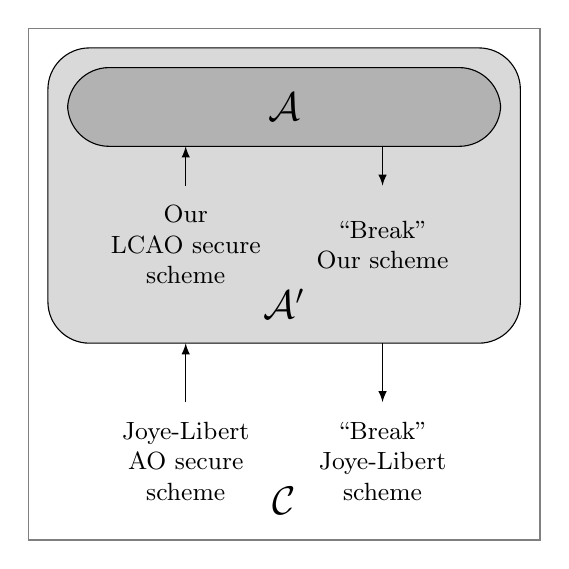
\begin{tikzpicture}[font=\small]
    % Bounding box
    \draw [gray] (0,0) rectangle (6.5,6.5);

    % Outer adversary rectangle
    \draw[rounded corners=15pt, fill=gray!30] (0.25,6.25) rectangle (6.25,2.5);
    % Inner adversary rectangle
    \draw[rounded corners=15pt, fill=gray!60] (0.5,6) rectangle (6,5);

    % Adversaries and challenger
    \node at (3.25,3) {\Large$\mathcal{A}'$};
    \node at (3.25,5.5) {\Large$\mathcal{A}$};
    \node at (3.25,0.5) {\Large$\mathcal{C}$};

    % Arrows
    \node[text width=3cm, align=center] at (2,1) {Joye-Libert\\AO secure\\scheme};
    \draw [-latex] (2,1.75) -- (2,2.5);

    \node[text width=3cm, align=center] at (2,3.75) {Our\\LCAO secure\\scheme};
    \draw [-latex] (2,4.5) --(2,5);

    \node[text width=3cm, align=center] at (4.5,3.75) {``Break''\\Our scheme};
    \draw [-latex] (4.5,5) -- (4.5,4.5);

    \node[text width=3cm, align=center] at (4.5,1) {``Break''\\Joye-Libert\\scheme};
    \draw [-latex] (4.5,2.5) -- (4.5,1.75);
\end{tikzpicture}